\section{Verificación}
Para validar el diseño se escribió el testbench \texttt{tb\_top.v}, que ejercita el módulo top completo (registros y ALU) de la misma forma en que se usaría la placa. Genera un reloj de 10~ns (igual al de la Basys 3), aplica un reset inicial y luego, para cada caso, carga A, B y el opcode en \texttt{i\_datos}, activando durante un ciclo el bit de \texttt{i\_abc} correspondiente a cada uno:

\begin{lstlisting}[caption={Carga de un caso en el testbench.}]
// Caso feliz: 20 + 22 = 42
@(negedge clock); i_datos = 8'd20; i_abc = 3'b001;
@(negedge clock); i_datos = 8'd22; i_abc = 3'b010;
@(negedge clock); i_datos = ADD;   i_abc = 3'b100;
@(negedge clock); i_abc = 3'b000;
#100;
\end{lstlisting}

Las entradas se modifican en el flanco de bajada del reloj para que estén estables cuando el módulo top las registra en el flanco de subida. Si se cambiaran en el mismo flanco de subida, el resultado dependería del orden en que el simulador evalúe los bloques (una condición de carrera). Entre caso y caso se dejan 100~ns para poder observar la salida en las formas de onda.

\subsection{Casos de prueba}
Además de un caso feliz, se eligieron casos extremos para cada operación: sumas y restas en los límites del rango representable en complemento a dos (donde aparece el \textit{overflow}), resultados nulos, operaciones lógicas con todos unos y todos ceros, desplazamientos máximos y un opcode inválido. Por último, se aplica un reset con los registros cargados para verificar que la salida vuelve a cero. La Tabla~\ref{tab:casos} resume los casos y los valores esperados, que se contrastaron con las formas de onda obtenidas.

\begin{table}[H]
	\centering
	\caption{Casos de prueba del testbench y resultados esperados.}
	\label{tab:casos}
	\begin{tabular}{lrrlrcc}
		\toprule
		\textbf{Op.} & \textbf{A} & \textbf{B} & \textbf{Caso} & \textbf{Resultado} & \textbf{Z} & \textbf{OV} \\
		\midrule
		ADD & 20 & 22 & Caso feliz & 42 & 0 & 0 \\
		ADD & 127 & 1 & Máximo positivo $+1$ & $-128$ & 0 & 1 \\
		ADD & $-128$ & $-1$ & Mínimo negativo $-1$ & 127 & 0 & 1 \\
		ADD & 127 & $-127$ & Opuestos & 0 & 1 & 0 \\
		SUB & $-128$ & 1 & Mínimo negativo $-1$ & 127 & 0 & 1 \\
		SUB & 127 & $-1$ & Máximo positivo $+1$ & $-128$ & 0 & 1 \\
		SUB & 0 & $-128$ & $+128$ no representable & $-128$ & 0 & 1 \\
		SUB & $-128$ & $-128$ & Iguales & 0 & 1 & 0 \\
		AND & \texttt{FF} & \texttt{00} & Todos ceros & \texttt{00} & 1 & 0 \\
		OR  & \texttt{F0} & \texttt{0F} & Complementarios & \texttt{FF} & 0 & 0 \\
		XOR & \texttt{FF} & \texttt{FF} & Iguales & \texttt{00} & 1 & 0 \\
		NOR & \texttt{00} & \texttt{00} & Todos ceros & \texttt{FF} & 0 & 0 \\
		SRA & \texttt{80} & 7 & Desplazamiento máximo & \texttt{FF} & 0 & 0 \\
		SRL & \texttt{80} & 7 & Desplazamiento máximo & \texttt{01} & 0 & 0 \\
		SRL & \texttt{FF} & 8 & Fuera de rango & \texttt{00} & 1 & 0 \\
		\texttt{111111} & 55 & 66 & Opcode inválido & 0 & 1 & 0 \\
		\bottomrule
	\end{tabular}
\end{table}

Los casos de SRA y SRL usan el mismo operando, \texttt{10000000} ($-128$), para poner en evidencia la diferencia entre ambos: el desplazamiento aritmético replica el bit de signo y da $-1$, mientras que el lógico completa con ceros y da 1.

\subsection{Resultados}
El testbench se ejecutó en simulación comportamental y en simulación temporal post-implementación. Esta última utiliza la netlist ruteada, con los retardos reales de cada celda y conexión. En ambas simulaciones las salidas coincidieron con los valores de la Tabla~\ref{tab:casos}. En la simulación post-implementación se observa además que la salida no cambia inmediatamente después del flanco de reloj, sino que tarda varios nanosegundos en estabilizarse, en concordancia con el análisis de tiempos de la Sección~\ref{sec:tiempos}.

La Figura~\ref{fig:testbench} muestra un fragmento de la simulación comportamental, entre los 880 y los 1060~ns aproximadamente, con los valores en hexadecimal. Se observan dos de los casos extremos de la resta:
\begin{itemize}
	\item \textbf{$127 - (-1)$:} se carga A = \texttt{7f} (\texttt{i\_abc} = 1) y luego B = \texttt{ff} (\texttt{i\_abc} = 2). Como el opcode sigue siendo SUB (\texttt{22}) del caso anterior, la salida cambia en cuanto se carga cada operando. Con A = 127 y el B anterior (1) se obtiene \texttt{7e} (126) sin \textit{overflow}. Al cargar B = $-1$, el resultado pasa a \texttt{80} ($-128$) y se activa \texttt{o\_overflow}, ya que $+128$ no es representable en 8 bits. Por último se vuelve a cargar el opcode (\texttt{i\_abc} = 4), sin cambios en la salida.
	\item \textbf{$0 - (-128)$:} al cargar A = \texttt{00}, la salida pasa a \texttt{01} ($0 - (-1)$) y el \textit{overflow} se desactiva. Al cargar B = \texttt{80} ($-128$), el resultado vuelve a ser \texttt{80} con \textit{overflow}, ya que nuevamente el resultado exacto sería $+128$.
\end{itemize}

\begin{figure}[H]
	\centering
	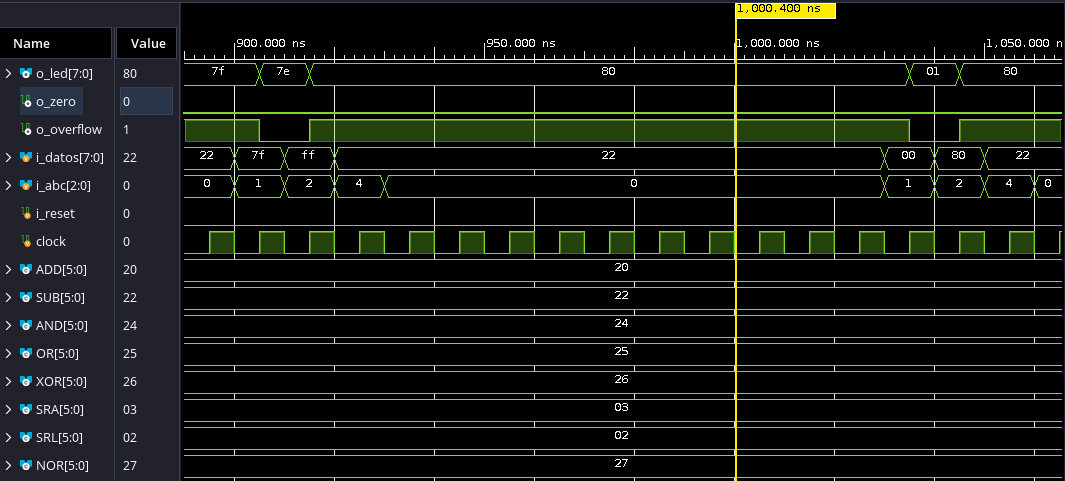
\includegraphics[width=\textwidth]{img/testbench.png}
	\caption{Formas de onda de la simulación comportamental: casos $127 - (-1)$ y $0 - (-128)$.}
	\label{fig:testbench}
\end{figure}

Esta captura también pone en evidencia el comportamiento del módulo top: como la ALU es combinacional y está conectada directamente a los registros, la salida refleja en todo momento la operación entre los valores cargados hasta ese instante, y se actualiza en el mismo flanco de reloj en que se carga cada registro.
